\section{The modelling side: shorter runs for the same answer}\label{sec:modelling}

Once the engine is at the bus, a run's wall time is cells $\times$ time steps $\div$ speed, and the first two are
set by the model and by openEMS's time-step criterion. Three changes act there; all live in the author's simulation
toolkit (rfsim) except the end criterion, which is in openEMS. The changes made to the toolkit in this project are not
published, since the toolkit itself is private; this section and \code{CHANGELOG.md} describe them.

\subsection{A run-end criterion on the port probes}\label{sec:probeend}
openEMS stops a run when the total field energy has fallen below a threshold relative to its peak (default
$-50$\,dB) or at a maximum number of steps or time. On both boards the energy criterion never fires: a Gaussian
pulse has a DC component, the open structure stores it as a static charge, and the energy stays far above the
threshold. At the end of the full runs of Table~\ref{tab:probeend} it still reads $-11.1$\,dB (SMA) and $-14.9$\,dB
(GCPW) of its peak (\code{results/rfsim\_e2e\_2026-11-03.txt}), while every port signal is below $-80$\,dB of its
peak after about a quarter of the run. Runs therefore always went to \code{max\_time}, and the toolkit proved
settling after the fact from the port files. Upstream master has since added an opt-in DC-free Gaussian pulse (commit
d686f1d, 2026-10-24: \code{SetGaussExcite(f0, fc, dc\_free=True)}, a sine instead of a cosine carrier); it is not in
v0.37.0 or in the fork's base. It leaves no static charge, so the energy criterion can fire, but it changes the
excitation: its spectrum falls to zero at DC, so the bottom of the band (50\,MHz for these boards) is driven more
weakly. The criterion below keeps the model and its pulse as they are.

The fork adds a second criterion, off unless \code{OPENEMS\_PROBE\_END\_DB} is set to a negative level in dB; an
invalid value of it or of \code{OPENEMS\_PROBE\_END\_HOLD} prints a warning. Every integral probe (port voltages and
currents, field probes) tracks the largest absolute value it has seen and its latest value; a waveguide
(mode-matching) probe counts with its mode amplitude only, not its mode purity. At every step at which one of the
processings runs (a probe or dump sample, or an energy estimate; on the GCPW line the probes sample every 490 steps, a
quarter of the Nyquist interval), the engine computes the worst ratio latest/peak over all probes, so a run can only
stop on such a step. It stops once that ratio has stayed below the threshold for a hold time of
\code{OPENEMS\_PROBE\_END\_HOLD} excitation lengths (default 1). The hold starts again at every check at which a
probe is above the threshold, a probe has seen no signal yet (its peak is still exactly zero), or the excitation is
still running; the excitation counts as running until the end of its signal plus the largest excitation delay, taken
over every grid (the child grids of a cylindrical multigrid included) and including the propagation delay of a
total-field/scattered-field (TFSF) source. A probe that never sees a signal holds the run to its end; once all the
others have settled, a one-time notice names it. A far probe can pick up tiny numerical precursors shortly before the
pulse arrives, and those count as a signal, so the hold should be longer than the longest one-way delay from the
excitation to a probe. A probe whose own peak is below $10^{-6}$ of the largest peak of its kind (a current probe on an
open end, say) is measured against $10^{-6}$ of that largest peak instead of its own near-zero peak. The criterion
needs a Gaussian excitation and at least one probe; if either is missing it prints a warning and ignores the setting.
The time-domain probe and port files of a stopped run are a bit-identical prefix of the full run's (checked for every
stopped run of Table~\ref{tab:probeend}; only the stop point changes); frequency-domain dumps and nf2ff data are sums
over the shorter record and change accordingly. The toolkit sets the variables around every \code{FDTD.Run()}: by
default \code{probe\_end\_db=-60} and, since toolkit commit 4a7e20e of 2026-11-04, \code{probe\_end\_hold=0.5}
(\code{RFSIM\_PROBE\_END\_HOLD=1} restores the earlier default of 1).
Table~\ref{tab:probeend} shows the effect on both boards.

\begin{table}[H]\centering\small
\resizebox{\textwidth}{!}{\begin{tabular}{@{}llrrl@{}}
\toprule
model & setting & steps & time & change vs the full run \\
\midrule
GCPW line, 12\,ns & full run (max\_time) & 94\,217 & 13.7\,s & -- \\
 & $-60$\,dB, hold 1 & 45\,570 & 8.6\,s & $S_{21}$ $8.0\times10^{-4}$\,dB, $S_{11}$ $1.3\times10^{-4}$ lin., $Z_0$ $-0.0003\,\Omega$ \\
 & $-80$\,dB, hold 1 & 47\,040 & 7.1\,s & $S_{21}$ $7.9\times10^{-4}$\,dB, $S_{11}$ $1.2\times10^{-4}$ lin., $Z_0$ $-0.0009\,\Omega$ \\
 & $-60$\,dB, hold 0.5 & 34\,300 & 5.2\,s & $S_{21}$ $7.1\times10^{-4}$\,dB, $S_{11}$ $2.2\times10^{-4}$ lin., $Z_0$ $-0.0005\,\Omega$ \\
\addlinespace
SMA launch, 10\,ns & full run (max\_time) & 182\,622 & 168.5\,s & -- \\
 & $-60$\,dB, hold 1 & 103\,831 & 97.6\,s & $S_{11}$ 0.0089\,dB at $-22.8$\,dB, $S_{21}$ $2.3\times10^{-4}$\,dB, $Z_0$ $-0.0066\,\Omega$ \\
 & $-80$\,dB, hold 1 & 106\,113 & 99.8\,s & $S_{11}$ 0.0100\,dB, $S_{21}$ $1.9\times10^{-4}$\,dB, $Z_0$ $-0.0037\,\Omega$ \\
 & $-60$\,dB, hold 0.5 & 77\,588 & 72.9\,s & $S_{11}$ 0.0188\,dB, $S_{21}$ $2.2\times10^{-4}$\,dB, $Z_0$ $-0.0092\,\Omega$ \\
\bottomrule
\end{tabular}}
\caption{Probe end criterion on the two boards: cg18, automatic thread count, one run each, measured on 2026-11-03
(\code{results/rfsim\_e2e\_2026-11-03.txt}); the SMA launch on the 1.071\,M-cell mesh of the toolkit's former
0.02\,mm floor ($\Delta t$ 54.76\,fs). On the GCPW line the $-60$\,dB, hold 0.5 row is the toolkit's
default run since 2026-11-04; on the SMA launch that default also has the 0.05\,mm mesh floor (Table~\ref{tab:mesh}).
Time: wall time of \code{FDTD.Run} (operator setup and time stepping). Changes against the
full run of the same board, the largest over 50\,MHz--2\,GHz: $|\Delta S_{21}|$ in dB; $|\Delta S_{11}|$ linear on the
GCPW line (its $S_{11}$ stays below $-40$\,dB) and in dB where $|S_{11}|>-40$\,dB on the SMA launch; $\Delta Z_0$ is
the change of $\mathrm{Re}\,Z_0$ at 640\,MHz (GCPW) and 1\,GHz (SMA). In the GCPW's $-60$\,dB, hold 1 run the tuner
picked 8 threads (1\,304\,\MC, against 1\,636--1\,683\,\MC\ at 4 threads in the other fdtdKit GCPW runs), so it took
longer than the $-80$\,dB run, which has more steps.}\label{tab:probeend}
\end{table}

\subsection{z lines in multiples of four}
The SSE engines pack four z lines per vector and compute $4n_v$ slots per $(x,y)$ column ($n_v=\lceil N_z/4\rceil$
z-vectors; the spare slots are the top lane of the last z-vectors), so a board with 17 z lines costs the time of 20.
The toolkit can now halve the largest z cell (the air above the board) until the line count is a multiple of four; it
never splits the boundary cells at z max (one for Mur, $N$ for PML\_$N$) and never shrinks the time step. The GCPW
line goes from 17 to 20 lines and from 0.242 to 0.285 million cells in the \emph{same} wall time (bench: 1.13\,s versus
1.10\,s for 8\,000 steps at 4 threads), with the time step unchanged. It is a finer mesh, so results move, by
$5\times10^{-5}$ relative in the probes and $10^{-4}$\,dB in $S_{21}$; it is opt-in. These numbers are from the
project log, not in \code{results/}, and were taken with the first version of the padding, which also split the top
boundary cell; the toolkit's current version keeps that cell, so its mesh differs at the top (the line count, and
with it the timing, is the same). Rounding down instead, by dropping the top-most air line (17 to 16 lines), would save one
z-vector of run time, but it lowers the lid by one air cell: a change of the model rather than of its mesh, left to
the toolkit's user.

\subsection{A minimum cell size for the SMA launch}\label{sec:meshfloor}
The SMA launch has 69\,500 distinct operators and, on the toolkit's original mesh (that of 2026-10-17), a time step
of 53.0\,fs set by cells of 0.025--0.045\,mm (operator count and cell sizes from the project log, the time step from
\code{results/sma\_mesh\_sweep\_2026-11-01.txt}). Those cells are not design intent: they are where a tangent line of
the pin, the PTFE bore or a via edge lands 0.025--0.045\,mm from a line of the regular 0.075 or 0.15\,mm grids. The
builder merged lines closer than 0.02\,mm by keeping the first; it now takes a \code{min\_cell} floor and merges with
priorities: strip and gap lines (the port's $1/3$--$2/3$ edge rule) always stay, a geometry line wins over a grid
line, and two geometry lines meet in the middle so the error is split. The first core cell under the top plane also
starts at the floor.

A first version of this merge was swept on 2026-11-01 (engine cg16, against the full run on the original mesh; the
first table of \code{results/sma\_mesh\_sweep\_2026-11-01.txt}). At 0.06\,mm the four-cell prepreg lost two of its
cells and $S_{11}$ moved by up to 3.3\,dB ($-19.98$ against $-22.80$\,dB at 1\,GHz); the last row of
Table~\ref{tab:mesh} keeps that run as history. The pre-publication review of this change then found two bugs in
that first merge. The floor was not multiplied by the model's \code{scale} factor, so the 0.6 convergence mesh was
merged with the unscaled floor and the coarse/fine pair was no longer a convergence pair; and the merge scanned the
lines from $-y$ to $+y$, so chains of three or more close lines resolved differently on the two sides and a
mirror-symmetric structure got an asymmetric mesh at every floor above 0.02\,mm. The merge is now independent of the
scan order (\code{core.merge\_lines}): protected lines never move and are never merged; a pair or a short run of
geometry lines closer than the floor is replaced by its mean, and a longer run (a grid finer than the floor) is
thinned to evenly spaced lines at least the floor apart; grid lines give way; and the builder refuses a floor that is
not below every fixed cell of the stack-up or the strip rule (0.0526\,mm and above for this board, 0.06\,mm included).

The 0.02\,mm mesh, the toolkit's default until 2026-11-04, is the same line for line with both merges; against
the original mesh it differs in the 14 lines that the caption of Table~\ref{tab:mesh} lists, and its time step is
54.76\,fs instead of 53.0\,fs. With the corrected merge the 0.04 and 0.05\,mm meshes gained lines (0.953 and 0.871
million cells; the first merge had dropped lines asymmetrically). A sweep of these meshes on 2026-11-02 ran while
other simulations loaded the machine, so its run times could only be estimated. Figure~\ref{fig:mesh} and
Table~\ref{tab:mesh} give the sweep measured on 2026-11-03 with cg18 and the corrected merge, against the full run on
the 0.02\,mm mesh; it reproduces the step counts of 2026-11-02 exactly and replaces the estimated
times. The suggestion stands: 0.05\,mm with a hold of 0.5 needs 2.54 times fewer cell-steps and 2.61 times less run
time than the earlier defaults (the 0.02\,mm mesh with a hold of 1; 37.4\,s against 97.6\,s), with $S_{11}$ within
0.12\,dB at $-22.8$\,dB and $Z_0$ 0.12\,$\Omega$ higher; with a hold of 1 the floor alone gives 1.90 and 1.97 times
(49.5\,s). That error is far inside the 30\,dB return-loss bench floor the model documents for itself: an error wave
30\,dB below the incident one, on a reflection of $-22.8$\,dB, allows any reading from $-19.7$ to $-27.8$\,dB. The
author adopted it on 2026-11-04: since toolkit commit 4a7e20e the toolkit's defaults are the 0.05\,mm floor
(0.871\,million cells on this board) and a hold of 0.5 for every run, and \code{RFSIM\_MIN\_CELL=0.02} and
\code{RFSIM\_PROBE\_END\_HOLD=1} restore the old ones.

\begin{table}[H]\centering\small
\resizebox{\ifdim\width>\textwidth\textwidth\else\width\fi}{!}{\begin{tabular}{@{}lrrrrrrr@{}}
\toprule
floor & cells & $\Delta t$ & steps & run & $S_{11}$ at 1\,GHz & $\max|\Delta S_{11}|$ / $|\Delta S_{21}|$ & $\Delta Z_0$ \\
\midrule
0.02\,mm$^{\dagger}$ & 1.071\,M & 54.8\,fs & 103\,831 & 97.6\,s & $-22.80$\,dB & 0.0089 / 0.0002\,dB & $-0.007$\,$\Omega$ \\
0.03\,mm & 1.007\,M & 58.5\,fs & 97\,097 & 85.7\,s & $-22.79$\,dB & 0.0292 / 0.0006\,dB & +0.03\,$\Omega$ \\
0.04\,mm & 0.953\,M & 78.0\,fs & 72\,891 & 58.0\,s & $-22.72$\,dB & 0.0782 / 0.0014\,dB & +0.12\,$\Omega$ \\
0.05\,mm & 0.871\,M & 84.4\,fs & 67\,340 & 49.5\,s & $-22.69$\,dB & 0.1156 / 0.0021\,dB & +0.10\,$\Omega$ \\
0.02\,mm, hold 0.5 & 1.071\,M & 54.8\,fs & 77\,588 & 72.9\,s & $-22.80$\,dB & 0.0188 / 0.0002\,dB & $-0.009$\,$\Omega$ \\
0.05\,mm, hold 0.5$^{*}$ & 0.871\,M & 84.4\,fs & 50\,320 & 37.4\,s & $-22.69$\,dB & 0.1157 / 0.0021\,dB & +0.12\,$\Omega$ \\
\midrule
\multicolumn{8}{@{}l@{}}{\emph{history: first merge, 2026-11-01 (engine cg16; see the caption)}} \\
0.06\,mm & 0.625\,M & 130.1\,fs & 43\,680 & 24.3\,s & $-19.98$\,dB & 3.292 / 0.0237\,dB & +0.43\,$\Omega$ \\
\bottomrule
\end{tabular}}
\caption{SMA launch mesh floor sweep, 10\,ns, probe end $-60$\,dB with a hold of 1 unless stated, measured on
2026-11-03 with cg18 (the tuner picked 8 threads in every run), one run each, with the corrected merge (the
2026-11-03 section of \code{results/sma\_mesh\_sweep\_2026-11-01.txt}; the same runs as in
\code{results/rfsim\_e2e\_2026-11-03.txt}). Run: wall time of \code{FDTD.Run}. Changes against the full run on the
0.02\,mm mesh (182\,622 steps of 54.76\,fs, Table~\ref{tab:probeend}): $\Delta S_{11}$ in dB where
$|S_{11}|>-40$\,dB over 50\,MHz--2\,GHz, $\Delta S_{21}$ the largest over that band, $\Delta Z_0$ the change of
$\mathrm{Re}\,Z_0$ at 1\,GHz (to 0.01\,$\Omega$ where it exceeds 0.01\,$\Omega$). $^{\dagger}$The toolkit's default
until 2026-11-04 (with a hold of 1). $^{*}$The toolkit's default since 2026-11-04 (toolkit commit 4a7e20e).
The first row's mesh differs from the toolkit's original mesh (that of 2026-10-17: 188\,697 steps of 53.0\,fs for
10\,ns) in 14 lines: nine move by at most 0.01\,mm (four in x, five in y) and five y lines between 3.6 and 4.45\,mm by
up to 0.10\,mm, where the original y mesh was not mirror-symmetric. The last row is history: the 0.06\,mm run of the
first merge (2026-11-01, against the full run on the original mesh; the first table of the same file), in which the
four-cell prepreg lost two of its cells; the builder refuses that floor now.}\label{tab:mesh}
\end{table}

\begin{figure}[htbp]\centering
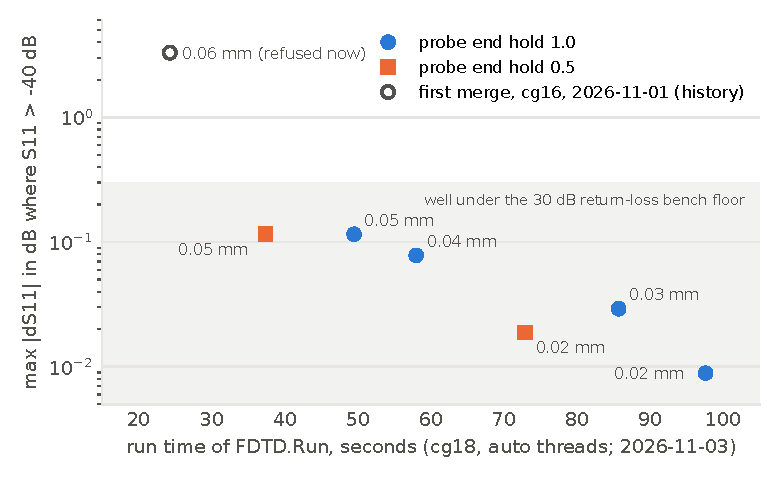
\includegraphics[width=0.62\textwidth]{fig_mesh}
\caption{Run time against the $S_{11}$ error for the mesh floors of Table~\ref{tab:mesh}, measured on 2026-11-03 with
cg18 and the corrected merge. The hollow grey point is history: the 0.06\,mm run of the first
merge (2026-11-01, engine cg16, against the full run on the original mesh), a floor the builder now
refuses.}\label{fig:mesh}
\end{figure}
